\documentclass[sigconf]{acmart}

\usepackage{booktabs} % For formal tables

\usepackage{etoolbox}
\usepackage{xstring}
\DeclareListParser{\doslashlist}{/}
\newcounter{ndnNameComponentCounter}%
\newcommand{\ndnName}[1]{{%
  \setcounter{ndnNameComponentCounter}{0}%
  \renewcommand{\do}[1]{{%
    \ifnumgreater{\value{ndnNameComponentCounter}}{0}{\allowbreak/}{}%
    \ifnumodd{\value{ndnNameComponentCounter}}{}{}%
    \detokenize{##1}}%
    \stepcounter{ndnNameComponentCounter}}%
``{\fontfamily{cmtt}\small\selectfont\IfBeginWith{#1}{/}{/}{}\doslashlist{#1}}''%
}}

\setcopyright{rightsretained}

\begin{document}
\title{Project Report: Virtual Organization Over Named Data Networking}
\titlenote{Produces the permission block, and
  copyright information}
\subtitle{Extended Abstract}
\subtitlenote{The full version of the author's guide is available as
  \texttt{acmart.pdf} document}

\author{Zhiyi Zhang}
\affiliation{%
  \institution{UCLA}
}
\email{zhiyi@cs.ucla.edu}

\author{Yukai Tu}
\affiliation{%
  \institution{UCLA}
}
\email{ytu@cs.ucla.edu}

% \author{Craig A. Lee}
% \affiliation{%
%   \institution{The Aerospace Corporation}
% }
% \email{lee@aero.org}

% \author{Alexander Afanasyev}
% \affiliation{%
%   \institution{UCLA}
% }
% \email{aa@cs.ucla.edu}

% \author{Lixia Zhang}
% \affiliation{%
%   \institution{UCLA}
% }
% \email{lixia@cs.ucla.edu}


% The default list of authors is too long for headers}
\renewcommand{\shortauthors}{Z. Zhang et al.}

\begin{abstract}

This paper provides a sample of a \LaTeX\ document which conforms,
somewhat loosely, to the formatting guidelines for
ACM SIG Proceedings.\footnote{This is an abstract footnote}

\end{abstract}

\keywords{Resource Sharing, Named Data Networking, Attribute-based Access Control}

\maketitle

\section{Introduction}

Resource sharing across the Internet has always been a need that is widely recognized for decades.
Yet, the isolation is still there and becomes a roadblock.
A large amount of efforts have been made to achieve collaboration and break the isolation.
However, it is still a big challenge to ensure the privacy, security, efficiency and semantic content at the same time.

Today, most resource sharing among multiple organizations, i.e. service provider, data producer, is done through the direct communication between two parties.
There is rarely or no collaboration platform that organize the resources from multiple organizations.
Also, the security and privacy of current resource sharing are usually ensured by following two mechanisms:
\begin{itemize}
\item \textbf{Protecting the communication channel} \\
Protocol like TLS encrypts the end-to-end channel to provide data exchange.
However, protecting channel always means to sacrifice the efficiency of content distribution.
For example, content multicast is not supported by channel-based security.
\item \textbf{Protecting the content} \\
There are mechanisms that provide encryption-based security.
For example, there are encryption-based access control systems using traditional asymmetric public key encryption or attribute-based encryption.
The content-based encryption allows the encrypted data to be stored publicly.
However, protecting content always means the lost of the semantic meaning.
For example, the resource sharing platform have no clue of the content and it's hard to organize millions of resources with blind eyes.
\end{itemize}

\section{Background}

\subsection{Tables}
Because tables cannot be split across pages, the best
placement for them is typically the top of the page
nearest their initial cite.  To
ensure this proper ``floating'' placement of tables, use the
environment \textbf{table} to enclose the table's contents and
the table caption.  The contents of the table itself must go
in the \textbf{tabular} environment, to
be aligned properly in rows and columns, with the desired
horizontal and vertical rules.  Again, detailed instructions
on \textbf{tabular} material
are found in the \textit{\LaTeX\ User's Guide}.

Immediately following this sentence is the point at which
Table~\ref{tab:freq} is included in the input file; compare the
placement of the table here with the table in the printed
output of this document.

\begin{table}
  \caption{Frequency of Special Characters}
  \label{tab:freq}
  \begin{tabular}{ccl}
    \toprule
    Non-English or Math&Frequency&Comments\\
    \midrule
    \O & 1 in 1,000& For Swedish names\\
    $\pi$ & 1 in 5& Common in math\\
    \$ & 4 in 5 & Used in business\\
    $\Psi^2_1$ & 1 in 40,000& Unexplained usage\\
  \bottomrule
\end{tabular}
\end{table}

To set a wider table, which takes up the whole width of the page's
live area, use the environment \textbf{table*} to enclose the table's
contents and the table caption.  As with a single-column table, this
wide table will ``float'' to a location deemed more desirable.
Immediately following this sentence is the point at which
Table~\ref{tab:commands} is included in the input file; again, it is
instructive to compare the placement of the table here with the table
in the printed output of this document.


\begin{table*}
  \caption{Some Typical Commands}
  \label{tab:commands}
  \begin{tabular}{ccl}
    \toprule
    Command &A Number & Comments\\
    \midrule
    \texttt{{\char'134}author} & 100& Author \\
    \texttt{{\char'134}table}& 300 & For tables\\
    \texttt{{\char'134}table*}& 400& For wider tables\\
    \bottomrule
  \end{tabular}
\end{table*}
% end the environment with {table*}, NOTE not {table}!

It is strongly recommended to use the package booktabs~\cite{Fear05}
and follow its main principles of typography with respect to tables:
\begin{enumerate}
\item Never, ever use vertical rules.
\item Never use double rules.
\end{enumerate}
It is also a good idea not to overuse horizontal rules.


\subsection{Figures}

Like tables, figures cannot be split across pages; the best placement
for them is typically the top or the bottom of the page nearest their
initial cite.  To ensure this proper ``floating'' placement of
figures, use the environment \textbf{figure} to enclose the figure and
its caption.

This sample document contains examples of \texttt{.eps} files to be
displayable with \LaTeX.  If you work with pdf\LaTeX, use files in the
\texttt{.pdf} format.  Note that most modern \TeX\ systems will convert
\texttt{.eps} to \texttt{.pdf} for you on the fly.  More details on
each of these are found in the \textit{Author's Guide}.

\begin{figure}
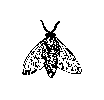
\includegraphics{fly}
\caption{A sample black and white graphic.}
\end{figure}

\begin{figure}
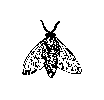
\includegraphics[height=1in, width=1in]{fly}
\caption{A sample black and white graphic
that has been resized with the \texttt{includegraphics} command.}
\end{figure}


As was the case with tables, you may want a figure that spans two
columns.  To do this, and still to ensure proper ``floating''
placement of tables, use the environment \textbf{figure*} to enclose
the figure and its caption.  And don't forget to end the environment
with \textbf{figure*}, not \textbf{figure}!

\begin{figure*}
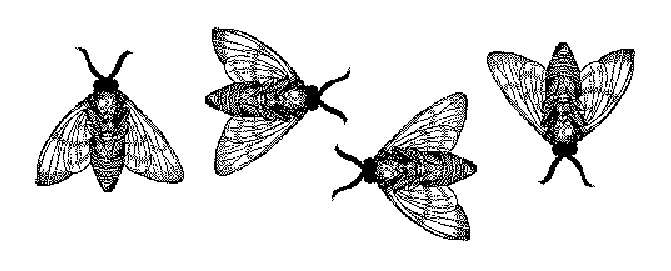
\includegraphics{flies}
\caption{A sample black and white graphic
that needs to span two columns of text.}
\end{figure*}


\begin{figure}
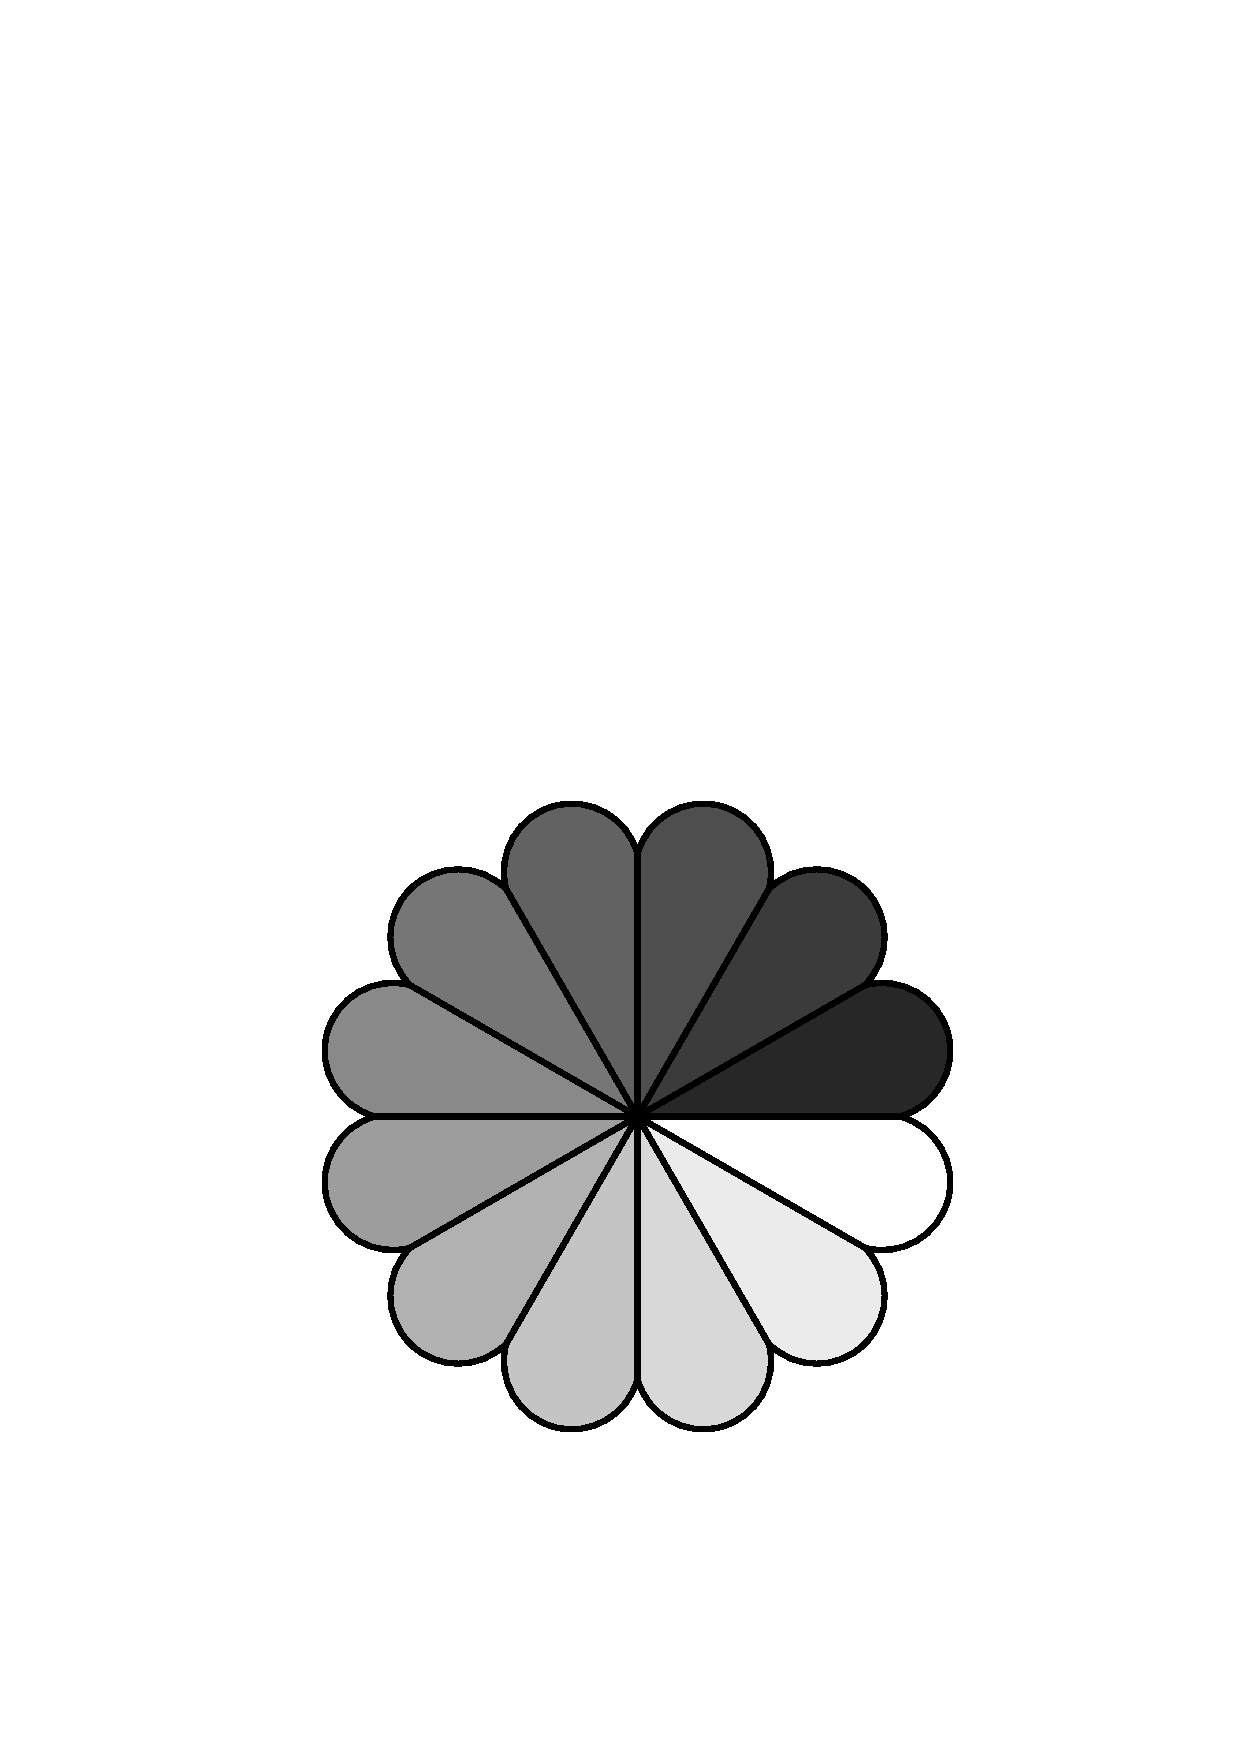
\includegraphics[height=1in, width=1in]{rosette}
\caption{A sample black and white graphic that has
been resized with the \texttt{includegraphics} command.}
\end{figure}

\subsection{Theorem-like Constructs}

Other common constructs that may occur in your article are the forms
for logical constructs like theorems, axioms, corollaries and proofs.
ACM uses two types of these constructs:  theorem-like and
definition-like.

Here is a theorem:
\begin{theorem}
  Let $f$ be continuous on $[a,b]$.  If $G$ is
  an antiderivative for $f$ on $[a,b]$, then
  \begin{displaymath}
    \int^b_af(t)\,dt = G(b) - G(a).
  \end{displaymath}
\end{theorem}

Here is a definition:
\begin{definition}
  If $z$ is irrational, then by $e^z$ we mean the
  unique number that has
  logarithm $z$:
  \begin{displaymath}
    \log e^z = z.
  \end{displaymath}
\end{definition}

The pre-defined theorem-like constructs are \textbf{theorem},
\textbf{conjecture}, \textbf{proposition}, \textbf{lemma} and
\textbf{corollary}.  The pre-defined de\-fi\-ni\-ti\-on-like constructs are
\textbf{example} and \textbf{definition}.  You can add your own
constructs using the \textsl{amsthm} interface~\cite{Amsthm15}.  The
styles used in the \verb|\theoremstyle| command are \textbf{acmplain}
and \textbf{acmdefinition}.

Another construct is \textbf{proof}, for example,

\begin{proof}
  Suppose on the contrary there exists a real number $L$ such that
  \begin{displaymath}
    \lim_{x\rightarrow\infty} \frac{f(x)}{g(x)} = L.
  \end{displaymath}
  Then
  \begin{displaymath}
    l=\lim_{x\rightarrow c} f(x)
    = \lim_{x\rightarrow c}
    \left[ g{x} \cdot \frac{f(x)}{g(x)} \right ]
    = \lim_{x\rightarrow c} g(x) \cdot \lim_{x\rightarrow c}
    \frac{f(x)}{g(x)} = 0\cdot L = 0,
  \end{displaymath}
  which contradicts our assumption that $l\neq 0$.
\end{proof}

\section{Security Model and Naming Convention}

\subsection{Ciphertext-policy Attribute-based Encryption over NDN}

\subsection{Naming Convention}

\section{Virtual Organization Over NDN}

\begin{figure*}[t]
  \centering
  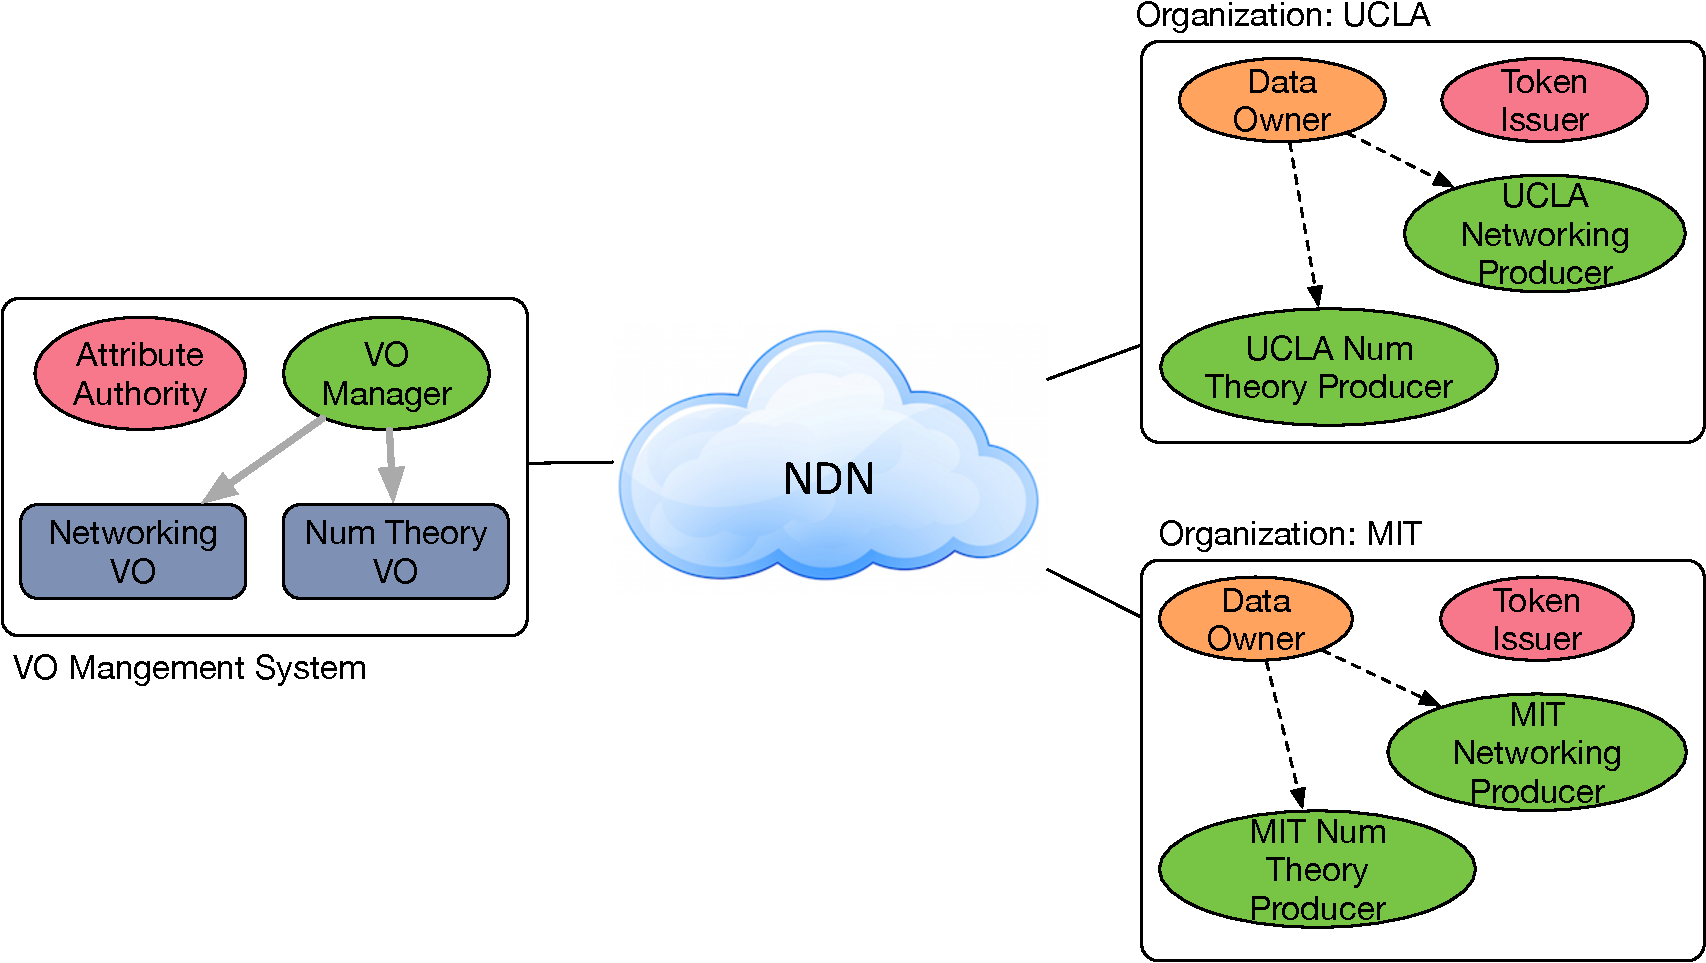
\includegraphics[scale=0.5]{figures/example}
  \vspace{-3mm}
  \caption{An example of how VO system work}
  \label{fig:example}
\end{figure*}

To facilitate explanation, in this section, we will use the following example (\ref{fig:example}) to illustrate the VO system.
The right side is the VO management system, which contains an \textbf{attribute authority} and a \textbf{VO manager}.
Attribute authority will setup the CPABE environment by generating public parameters and a secret master key.
The VO manager will create the VO, the data packet(s) containing the name category.
Both UCLA and MIT will produce networking lecture data and Number-theory lecture data.
There are two real-world organizations in our example: UCLA and MIT.
Besides producers which are the green circles, each organization also contains one \textbf{data owner} and one \textbf{token issuer}.
Data owner is the one who define the access rules for producer.
Token issuer takes the duty to help attribute authority to verify consumer's identity.

In NDN, each party is supposed to have an identity.
To make the example clear, we have the name like:

\begin{verbatim}
VO attribute authority: /vo/authority
VO manager: /vo/manager

UCLA token issuer: /ucla/token-issuer
UCLA data owner: /ucla/data-owner
UCLA network producer: /ucla/network
UCLA number theory producer: /ucla/num-theory
\end{verbatim}

In our example, there are also two VOs containing networking lecture data names and number theory lecture data names respectively.
In this way, the authorised consumers could easily access the networking/number theory lecture data both from UCLA and MIT through VO.

\subsection{VO Mangement System}

VO management system mainly contains two parts: attribute authority and VO manager.
The attribute authority will take the duty to setup the CPABE environment and issue decryption key for authorised consumers.
The VO manager will collect data information from each organization and produce VOs.

\subsubsection{Attribute Authority}
The attribute authority (AA) is a globally trust anchor.
All parties, no matter producer or consumer, should all trust the authority.
However, the existence of attribute authority won't lower down the security of the whole system and attribute authority won't become the single point of failure when system is running.
In the VO system, the attribute authority only works at the preliminary phase.
Once finish the system setup, the attribute authority should go offline to avoid potential attack from outside.

Before the system start running, AA would generate the public parameters which is a data packet and a secret master key.
In our system, the public parameter has the naming convention \texttt{/[AA-prefix]/PUB/<timestamp>}.
For instance, in the example, a possible name can be \texttt{/vo/authority/PUB/201706151200}.
The public parameters data packet will be signed by VO management system's certificate.
Regarding the master key, once the secret master key get compromised, the system will be broken.
In the preliminary phase, the authority will also issue consumer's decryption key based on the information provided by the token issuer.
The detail will be illustrated in the section \ref{token-issuer}.
This makes sure that the AA will only talk with trusted parties during the preliminary phase.

Once the system starts running, the AA should go offline immediately.
In the future, the AA should be awaken only when consumer's key get compromised and when there are new attributes.
Notice, even when AA is working, AA only needs to talk with token issuer, which is trusted.
If the token issuer corrupts, there is no security in system; thus only trustworthy party, like universities, government departement and etc., can become token issuer.

\subsubsection{VO Manager}
VO manager is the service provider who define the name category and produce VO packets.
All the organizations who wants to join the VO are supposed to provide the data information for VO manager.
The information should at least contains the data name and a category suggestion.
VO manager can use the application-readable data name to put each name into one or more VOs.

To protect the category information from unauthorized users, the data content should be encrypted by specific attribute.
In our system, there are VO attributes: "VO-001", "VO-002" and etc.
This kind of attribute is used to encrypt the name category.
Only user who has the corresponding key could see the category.
Notice that even users can see the category, it does not mean that users could consume the data for the data packets are encrypted by organization's policies.
For instance, assume the network lecture VO's data name is \texttt{/ucla/network/lesson1}

Each VO data packet

\subsection{Organization}

\subsubsection{Producer}

\subsubsection{Data Owner}

\subsubsection{Token Issuer} \label{token-issuer}


\subsection{Consumer}
\section{Implementation}

To see whether the design works or not under NDN environment, we implemented the Attribute-based Access Control Over NDN (ABAC-NDN) in C++ and corresponding test cases to verify it. ABAC-NDN is a complete C/C++ library with unit tests and integrate tests. There are more than 3500 lines of code (without copyright). It combines the AES, RSA and ABE encryption/decryption. The code depends on the ndn-cxx:, the basic NDN library, and Libbswabe, the CPABE support.

\subsection{ABAC-NDN code base}

There are five main components in the code base: Attribute Authority, Data Owner, Token Issuer, Consumer and Producer, shown in Fig.\ref{}.

When initializing the Attribute Authority, the public parameters and master key will be generated and uniquely used in global. All components except Token Issuer and Data Owner need to fetch public parameters for encryption and decryption. Besides, the Attribute Authority also registers the prefix to serve the decryption key request. All decryption keys will be generated for different users which will be verified and issued tokens. Since Attribute Authority trusts the Token Issuer, the token issued to a user will be verified and corresponding decryption key will be sent back to the user.

The Token Issuer and Data Owner are usually in the site-admin node. The Token Issuer is in charge of authorizing users. If the user is the member of that site-admin, the site-admin can verify it and issue the token for that user. The token is presented in JSON format. The Data Owner in charge of managing content produced by the producer under the site-admin. To define the rule for a certain data produced by a certain producer, the Data Owner express the Interest contains the producer prefix, data prefix and policy. The producer with that producer prefix receives that Interest and add the certain rule for that data.

The Producer and Consumer are corresponding to the encryption and decryption of the content. For Producer, when policy is set to a certain data, the Producer encrypts the content using public parameter and policy. The policy is in the form: $n$ attr1 to attrn mofn [attr2 to attrk jofk], where $m<=n$ and $j<=k$. It is the tree hierarchy structure which accepts any combination of the attributes. For example: attr1 attr2 1of2 attr3 2of2. Only who with attr1 or attr2 and at the same time with attr3 can decrypt the content encrypted by the above policy. To decrypt the content from the producer, the consumer first need to fetch the token from the Token Issuer which the producer belongs to. Then using the token to fetch the corresponding decryption key. If the decryption is created by the attributes satisfy the policy, with the public parameters, the content can be decrypt correctly.

\subsection{Test cases}
For now we verify the correctness of the ABAC-NDN using both unit tests and integrated tests. For unit test, all unit function in different components will be verified. And in integrated test, the whole work flow is tested and the consumer with correct attributes can decrypt the content and the consumer with insufficient attributes will be blocked from the content.
\section{Discussion}

The \textit{proceedings} are the records of a conference.\footnote{This
  is a footnote}  ACM seeks
to give these conference by-products a uniform, high-quality
appearance.  To do this, ACM has some rigid requirements for the
format of the proceedings documents: there is a specified format
(balanced double columns), a specified set of fonts (Arial or
Helvetica and Times Roman) in certain specified sizes, a specified
live area, centered on the page, specified size of margins, specified
column width and gutter size.

\section{Future Work}

Citations to articles~\cite{bowman:reasoning,
clark:pct, braams:babel, herlihy:methodology},
conference proceedings~\cite{clark:pct} or maybe
books \cite{Lamport:LaTeX, salas:calculus} listed
in the Bibliography section of your
article will occur throughout the text of your article.
You should use BibTeX to automatically produce this bibliography;
you simply need to insert one of several citation commands with
a key of the item cited in the proper location in
the \texttt{.tex} file~\cite{Lamport:LaTeX}.
The key is a short reference you invent to uniquely
identify each work; in this sample document, the key is
the first author's surname and a
word from the title.  This identifying key is included
with each item in the \texttt{.bib} file for your article.

The details of the construction of the \texttt{.bib} file
are beyond the scope of this sample document, but more
information can be found in the \textit{Author's Guide},
and exhaustive details in the \textit{\LaTeX\ User's
Guide} by Lamport~\shortcite{Lamport:LaTeX}.
\section{Conclusion}

In this paper, we proposed the Attribute-based Access Control over NDN which achieves the secure access control protocol over the NDN. The proposed ABAC-NDN includes the following advanced features:

\begin{itemize}
	\item Semi-distributed system.
	\item Asynchronous data production and consumption.
	\item Decoupled access control and knowledge of the consumers.
	\item Allow data owner and producer in different devices.
	\item Allow attribute authority and token issuer in different devices.
	\item Any party could become a producer immediately.
\end{itemize}

Compare to other encryption method in NDN, the ABAC is more feasible and more flexible. The attribute based encryption can serve NDN application in a good way, since the build-in distribution support in NDN can let consumer fetch the content based on Name and decrypt with attributes without other information like location in TCP/IP network. By encrypting and decrypting content based on the attributes, it can achieve the virtual organization concept we proposed in this paper.

With above advance features, we implemented the ABAC-NDN in a C++ library. The library can support the ABAC based application in NDN in an easy way. For now the unit tests and integrated test can verify the correctness of the proposed ABAC-NDN. It shows that our code base can successfully achieve the concept of virtual organization based on the attributes.


\bibliographystyle{ACM-Reference-Format}
\bibliography{ndn-abac-vo}

\end{document}
